\documentclass{article}

\usepackage{coursenotes}

\set{AuthorName}{TC Fraser}
\set{Email}{tcfraser@tcfraser.com}
\set{Website}{www.tcfraser.com}
\set{ClassName}{Applied Probability}
\set{School}{University of Waterloo}
\set{CourseCode}{Stat 333}
\set{InstructorName}{Yi Shen}
\set{Term}{Fall 2016}
\set{Version}{1.0}

\draftprofile[TC Fraser]{TC}{Purple}
\newcommand{\val}[1]{X_{#1} = x_{#1}}
\newcommand{\indep}{\!\!\perp\!\!\!\!\perp\!\!}
\newcommand{\Cov}{\textsf{Cov}}
\newcommand{\Var}{\textsf{Var}}
\newcommand{\Exp}{\mathbb{E}}
\newcommand{\Ber}{\mathsf{Ber}}
\newcommand{\Bi}{\mathsf{Bin}}
\newcommand{\Poi}{\mathsf{Poi}}
\newcommand{\Ex}{\mathsf{Exp}}
\newcommand{\Mom}{M}
\newcommand{\Geo}{\mathsf{Geo}}
\newcommand{\ind}{\mathbf{1}}

\begin{document}

\titlePage

\tableOfContents

\disclaimer

\section{Review}

If $X \indep Y$ then $\Cov\br{X,Y} = 0$ and,
\[ \Var\br{X+Y} = \Var\br{X} + \Var\br{Y} \]
We see that independence implies uncorrelated, but uncorrelation does not imply independence.

\begin{remark}
    We have that,
    \[ \Exp\br{X + Y} = \Exp\br{X} + \Exp\br{Y} \eq \label{eq:r11}\]
    If $X\indep Y$ then we also have that,
    \[ \Exp\br{XY} = \Exp\br{X}\Exp\br{Y} \eq \label{eq:r21}\]
    and that,
    \[ \Var\br{XY} = \Var\br{X}\Var\br{Y} \eq \label{eq:r22}\]
    It is important to remember that the first result (\cref{eq:r11}) and the other two results (\cref{eq:r21,eq:r22}) have a very different natures. The first is a consequence of the linearity in the definition of expectation and holds unconditionally. However \cref{eq:r21,eq:r22} require that $X \indep Y$. As such it is more appropriate to consider \cref{eq:r21,eq:r22} as properties of independence rather than the properties of expectation and variance.
\end{remark}

\subsection{Indicator}

A r.v. $\ind$ is called an \term{indicator} for an event $A$ if,
\[ \ind_A \br{\w} = \begin{cases}
    1 & \w \in A \\
    0 & \w \not\in A
\end{cases} \]

The most important property of the indicator random variable is that the expectation of $\ind_A$ is the same as the probability of the event $A$,
\[ \Exp\br{\ind_{A}} = P\br{A} \]
\begin{proof}
    Since $\ind_A$ is a Bernoulli random variable, the proof is easy. Consider,
    \begin{align*}
    P\br{\ind_A = 1} &= P\br{\bc{\w: \ind_A\br{\w} = 1}} \\
    &= P\br{\bc{\w: \w \in A}} \\
    &= P\br{A}
    \end{align*}
    Therefore the expectation of $\ind_A$ must be,
    \[ \Exp\br{\ind_A} = 1 \cdot P\br{\ind_A = 1} + 0 \cdot P\br{\ind_A = 0} = P\br{\ind_A = 1} = P\br{A} \]
\end{proof}

\begin{example}
    We see $\ind_A$ is just a Bernoulli random variable,
    \[ \ind_A \sim \Ber\br{P\br{A}} \]
\end{example}

\begin{example}
    Let $X \sim \Bi\br{n,p}$; $X$ is the number of successes in $n$ Bernoulli trials, each with a probability $p$ of success.
    \[ X = \ind_1 + \cdots + \ind_n \eq \label{eq:binary}\]
    Where $\bc{\ind_1, \ldots, \ind_n}$ are indicators for independent events. $\ind_i = 1$ if the $i$-th trial is a success and $\ind_i = 0$ if the $i$-th trial is a failure. Hence, $I_i$ are \term{iid} (independent and identically distributed) r.v.s. It is known that the expectation of $X$ is given by,
    \[ \Exp\br{X} = \sum_{k=0}^{n} k \begin{pmatrix}
        n \\ k
    \end{pmatrix} p^k \br{1-p}^{n-k} \]
    However \cref{eq:binary} yields the following approach,
    \begin{align*}
    \Exp\br{X} &= \Exp\br{\ind_1 + \cdots + \ind_n} \\
    &= \Exp\br{\ind_1} + \cdots + \Exp\br{\ind_n} \\
    &= n\Exp\br{\ind_1} \\
    &= np
    \end{align*}
    Moreover,
    \begin{align*}
    \Var\br{X} &= \Var\br{\ind_1 + \cdots + \ind_n} \\
    &= \Var\br{\ind_1} + \cdots + \Var\br{\ind_n} \note{Independence}\\
    &= n\Var\br{\ind_1} \\
    &= np\br{1-p}
    \end{align*}
    The variance $\Var\br{I_1}$ is given by,
    \[ \Var\br{I_1} = \Exp\br{I_1^2} - \br{\Exp\br{I_1}}^2 \]
    But notice that $I_1^2 = I_1$ is idempotent. Therefore,
    \[ \Var\br{I_1} = p - p^2 = p\br{1-p} \]
\end{example}
\begin{example}
    Let $X$ be a r.v. taking values in non-negative integers $\bc{0,1,2\ldots}$. Then we find that the expectation of $X$ is given by,
    \[ \Exp\br{X} = \sum_{n=0}^{\inf} P\br{X > n} \]
    Note that,
    \[ X = \sum_{n=0}^{\inf} \ind_n \]
    Where notationally $\ind_n \defined \ind_{\bc{X > n}}$. The intuition being that if $X = 3$, then $X = 1 + 1 + 1$ since $X = \underbrace{\ind_0 + \ind_1 + \ind_2}_3 + \underbrace{\ind_3}_0 + \ldots$.
    \begin{align*}
        \Exp\br{X} &= \Exp\br{\sum_{n=0}^{\inf} \ind_n} \\
        &= \sum_{n=0}^{\inf}\Exp\br{\ind_n} \note{Fubini's Theorem} \\
        &= \sum_{n=0}^{\inf}P\br{X > n} \\
    \end{align*}
\end{example}
\begin{example}
    In particular let $X \sim \Geo\br{p}$ where $\Exp\br{X} = \sum_{k=0}^{\inf} k \br{1-p}^{k-1} p$. More easily we have seen that $P\br{X > n} = \br{1 - p}^n$. Therefore by the geometric series,
    \[ \Exp\br{X} = \sum_{n=0}^{\inf}P\br{X>n} = \sum_{n=0}^{\inf} \br{1-p}^n = \f{1}{1 - \br{1-p}} = \f{1}{p} \]
\end{example}

\subsection{Moment Generating Function}

\begin{definition}
    \label{def:moment_generator}
    Let $X$ be a r.v. Then the function,
    \[ \Mom\br{t} = \Exp\br{e^{tX}} \eq \label{eq:moment_generator} \]
    is called the \term{moment generating function (mgf)} if $X$ if the expectation exists for all $t \in \br{-h, h}$ for some $h > 0$.
\end{definition}

\begin{remark}
    The moment generating function $\Mom$ is not always defined. It is important to check the existence of the expectation. \\
    To compensate this, the latter condition  in \cref{def:moment_generator} is necessary because the expectation $\Exp\br{e^{tX}}$ might not always exist for some $t$. Also notice that $\Mom\br{0} = 1$ always.
\end{remark}

We will now discuss some important properties of the moment generating function.
\begin{theorem}
    The moment generating function generates moments. For $t = 0$,
    \[ \Mom\br{0} = 1 \]
    Also,
    \[ \Mom^{(k)} \br{0} \defined \f{\dif^k}{\dif t^k} \Mom\br{t}\mid_{t=0} \]
    Has the nice property,
    \[ \Mom^{(k)} \br{0} = \Exp\br{X^k} \]
\end{theorem}
\begin{proof}
    Evidently,
    \[ \Mom\br{0} = \Exp\br{e^{0\cdot X}} = \Exp\br{1} = 1 \]
    Moreover,
    \begin{align*}
        \Mom^{(k)} \br{0} &= \f{\dif^k}{\dif t^k} \Mom\br{t}\mid_{t=0} \\
        &= \f{\dif^k}{\dif t^k} \Exp\br{e^{tX}}\mid_{t=0} \\
        &= \Exp\br{\f{\dif^k}{\dif t^k} e^{tX}\mid_{t=0}} \note{Dominant convergence theorem.} \\
        &= \Exp\br{X\f{\dif^{k-1}}{\dif t^{k-1}} e^{tX}\mid_{t=0}} \\
        &= \cdots \\
        &= \Exp\br{X^k e^{tX}\mid_{t=0}} \\
        &= \Exp\br{X^k}
    \end{align*}
\end{proof}
As a result Taylor series gives,
\begin{align*}
    M\br{t} &= \sum_{k=0}^{\inf} \f{M^{(k)}\br{0}}{k!}t^k \\
    &= \sum_{k=0}^{\inf} \f{\Exp\br{X^k}}{k!}t^k \\
\end{align*}
Which is a method that can be used to obtain the moment of a mgf.
\begin{theorem}
    \label{thm:sum_mgf}
    Let $X\indep Y$ with mgfs $\Mom_x$ and $\Mom_y$ be respective mgfs. Let $\Mom_{X+Y}$ be the mgf of $X+Y$. Then,
    \[ \Mom_{X+Y} = \Mom_X\Mom_Y \]
\end{theorem}
\begin{proof}
    \begin{align*}
        \Mom_{X+Y}\br{t} &= \Exp\br{e^{t\br{X+Y}}} \\
        &= \Exp\br{e^{tX}e^{tY}} \\
        &= \Exp\br{e^{tX}}\Exp\br{e^{tY}} \note{Independence} \\
        &= \Mom_X\br{t} \Mom_Y\br{t}
    \end{align*}
\end{proof}

\begin{theorem}
    \label{thm:same_dist}
    The moment generating function \textit{completely} determines the distribution of a r.v.
    \[ M_X\br{t} = M_Y\br{t} \quad \forall t \in \br{-h, h} \]
    For some $h > 0$, then
    \[ X \stackrel{d}{=} Y \]
    Which denotes that the random variables have the same distribution.
\end{theorem}

How can the moment generating function help?

\begin{example}
    Let $X \sim \Poi\br{\la_1}$ and $Y \sim \Poi\br{\la_2}$ where $X \indep Y$. Find the distribution of $X+Y$.\\
    To answer this, first derive the moment generating function of a Poisson distribution.
    \begin{align*}
        M_X\br{t} &= \Exp\br{e^{tX}} \\
        &= \sum_{n=0}^{\inf} e^{tn} P\br{X = n} \\
        &= \sum_{n=0}^{\inf} e^{tn} \f{\la_1^n}{n!} e^{- \la_1} \\
        &= e^{- \la_1}\sum_{n=0}^{\inf} \f{\br{e^{t}\la_1}^n}{n!}  \\
        &= e^{- \la_1}e^{\br{e^{t}\la_1}} \note{Taylor series}  \\
        &= e^{\la_1\br{e^{t}- 1}}  \\
    \end{align*}
    Likewise, $M_Y\br{t} = e^{\la_2\br{e^{t} - 1}}$. Therefore since $X \indep Y$,
    \[ M_{X+Y}\br{t} = M_X\br{t}M_Y\br{t} = e^{\br{\la_1 + \la_2}\br{e^{t} - 1}} \]
    Therefore by \cref{thm:same_dist}, the distribution of $X+Y$ is the same distribution as $\Poi\br{\la_1 + \la_2}$.
\end{example}

In general, if $X_1, X_2, \ldots, X_n$ are independent and $X_i \sim \Poi\br{\la_i}$, then,
\[ \sum_{i=1}^{n} X_i \sim \Poi\br{\sum_{i=1}^{n} \la_i} \]

\begin{definition}
    Moreover, we define the \term{joint moment generating function (jmgf)} for $X, Y$ random variables to be,
    \[ \Mom\br{t_1, t_2} = \Exp\br{e^{t_1 X + t_2 Y}} \]
    Provided that the expectation exists for $t_1 \in \br{-h_1, h_1}$ and $t_2 \in \br{-h_2, h_2}$ for $h_1, h_2 > 0$.
\end{definition}
Evidently, the joint moment generating function can be defined for any number of random variables. More generally, we can define the joint moment generating function with parameters $t_1, \ldots, t_n$ to be,
\[ \Mom\br{t_1, \ldots, t_n} = \Exp\br{\exp\br{\sum_{i=1}^{n} t_i X_i}} \]
For r.v.s $X_1, \ldots, X_n$ provided that the expectation exists for $t_i \in \br{-h_i, h_i}$ for some $h_i > 0$ for $i = 1, \ldots, n$. There are some nice properties of the jmgf. First, it should be possible to obtain the mgf from a particular r.v. $X_i$ from the jmgf which includes $X_i$.\\

Notice that,
\[ \Mom_X\br{t} = \Exp\br{e^{tX}} = \Exp\br{e^{t\cdot X + 0\cdot Y}} = M_{XY}\br{t, 0} \]

Another property of the jmgf is,
\[ \f{\di^{m+n}}{\di t_1^m \di t_2^n} M\br{t_1, t_2} \mid_{0,0} = \Exp\br{X^m Y^n} \]
The proof being very similar to the single r.v. case.

Thirdly, we have that if $X \indep Y$, then,
\[ \Mom\br{t_1, t_2} = \Mom_{X}\br{t_1}\Mom_{Y}\br{t_2} \eq \label{eq:seperable_indep}\]

\begin{proof}
    \begin{align*}
        \Mom\br{t_1, t_2} &= \Exp\br{e^{t_1 X + t_2 Y}} \\
        &= \Exp\br{e^{t_1 X}e^{t_2 Y}} \\
        &= \Exp\br{e^{t_1 X}}\Exp\br{e^{t_2 Y}} \note{Independence}\\
        &= \Mom_X\br{t_1}\Mom_Y\br{t_2}
    \end{align*}
\end{proof}
\begin{remark}
    It is important not to confuse this result with \cref{thm:sum_mgf}. The difference being that \cref{thm:sum_mgf} is a single argument mgf while \cref{eq:seperable_indep} is a multi-parameter function,
    \[ \Mom_{X+Y}\br{t} \neq M_{X,Y}\br{t_1, t_2} \]
    Therefore knowing that $\Mom_{X+Y}\br{t}$ is separable does not imply that $X \indep Y$. \cref{eq:seperable_indep} is a stronger statement than \cref{thm:sum_mgf}.
\end{remark}

\section{Conditional Distribution and Conditional Expectation}
\subsection{Conditional Distribution}
We first begin with the discrete case.
\begin{definition}
    Let $X$ and $Y$ ne discrete r.v.s. Then the \term{conditional distribution} of $X$ given $Y$ is given by,
    \[ P\br{X=x\mid Y=y} = \f{P\br{X=x, Y=y}}{P\br{Y=y}} \]
    We read this as the probability of the event $\bc{X = x}$ given that $\bc{Y=y}$ holds. We can also write this as a conditional pmf,
    \[ f_{X\mid Y=y}\br{x} \quad \text{or} \quad f_{X\mid Y}\br{x \mid y} \]
\end{definition}

The conditional probability is a legitimate pmf. First note that as required,
\[ f_{X \mid Y=y}\br{x} \geq 0 \quad \forall x \]
Also it should be clear that,
\[ \sum_{x}f_{X \mid Y=y}\br{x} = 1 \]
In fact, $P\br{Y=y}$ acts a \textit{normalization constant} for the probabilities $\sum_{x} P\br{X=x, Y=y}$. Note that given $Y=y$, as $X$ changes, the value of the function $f_{X \mid Y=y}\br{x}$ is proportional to the joint probability $P\br{X=x, Y=y}$.
\[ f_{X \mid Y=y}\br{x} \propto P\br{X=x, Y=y} \eq \label{eq:prop_cond}\]
Namely the proportionality constant is of course $\br{P\br{Y=y}}^{-1}$. Although easy to understand, \cref{eq:prop_cond} can be used to solve problems where the denominator $P\br{Y=y}$ is difficult to find.

\begin{example}
    Let $X_1 \sim \Poi \br{\la_1}$ and $X_2 \sim \Poi \br{\la_2}$ such that $X_1 \indep X_2$ and $Y = X_1 + X_2$. Then we can find $P\br{X_1 = k \mid Y = n} = f_{X \mid Y = y}\br{k}$ using the following process. Notice that $f_{X \mid Y = y}\br{k}$ can only be non-zero when $0 \leq k \leq n$ in order for $Y = X_1 + X_2$. In this case for fixed $n$,
    \[ P\br{X_1 = k \mid Y = n} = \f{P\br{X_1 = k, Y = n}}{P\br{Y = n}} \propto P\br{X_1 = k, Y = n} \]
    But since $Y = X_1 + X_2$ it must be that,
    \begin{align*}
    P\br{X_1 = k \mid Y = n} &\propto P\br{X_1 = k, X_2 = n - k} \\
    &= e^{-\la_1} \f{\la_1^k}{k!}e^{-\la_2} \f{\la_2^{n-k}}{\br{n-k}!} \\
    &\propto \f{\la_1^k}{k!}\f{\la_2^{-k}}{\br{n-k}!} \eq \label{eq:star}
    \end{align*}
    If we want to find the exact proportionality constant for \cref{eq:star}, we simply need to normalize $P\br{X_1 = k \mid Y = n}$ by summing over all values of $k$ in \cref{eq:star},
    \[ P\br{X_1 = k \mid Y=n} = \f{\la_1^k}{k!}\f{\la_2^{-k}}{\br{n-k}!}\bc{\f{\la_1^k}{k!}\f{\sum_{k=0}^{n}\la_2^{-k}}{\br{n-k}!}}^{-1} \]
    Proceeding using this technique is difficult because of the nasty summation. The easier way is to continue the proportionality analysis. Compare \cref{eq:star} with the known result for common distributions. In particular, let's consider $X \sim \Bin\br{n, p}$,
    \[ P\br{X=k} = \begin{pmatrix}n\\k\end{pmatrix} p^k \br{1-p}^{n-k} = \f{n!}{k!\br{n-k}!} p^k \br{1-p}^{n-k} \]
    Removing constants,
    \[ P\br{X=k} \propto \br{\f{p}{1-p}}^k \br{k! \br{n-k}!}^{-1} \]
    Choosing $p/\br{1-p} = \la_1/\la_2$, then,
    \[ P\br{X_1 = k \mid Y = n} \propto P\br{X=k} \]
    Therefore we can conclude that $P\br{X_1 = k \mid Y = n}$ follows a binomial distribution with parameters $n$ and $p$ given by,
    \[ \f{p}{1-p} = \f{\la_1}{\la_2} \implies p = \f{\la_1}{\la_1 + \la_2}\]
    Therefore,
    \[ P\br{X_1 = k \mid Y = n} = \begin{pmatrix}n\\k\end{pmatrix} \br{\f{\la_1}{\la_1 + \la_2}}^k \br{1-\br{\f{\la_1}{\la_1 + \la_2}}}^{n-k} \]
\end{example}

We introduce the following notation. Denoted $X,Y \mid \bc{Z = k} \stackrel{\text{iid}}{\sim}\cdots$, this means that $X$ and $Y$ are \term{conditionally independent} and follows a certain distribution. i.e. the conditional joint cdf/pmf/pdf equals to the product of conditional (marginal) cdfs/pmfs/pdfs.

\subsection{Conditional Expectation}
We have seen that conditional pmf/pdf are legitimate pmf/pdf. Correspondingly, a conditional distribution is nothing else but a probability distribution. It is simply a potentially different distribution from the original unconditional distribution, since it takes more information into account. \\

As a result, we can define everything which are previously defined for unconditional distributions for conditional distributions. In particular, it is natural to define the conditional expectation as follows.
\begin{definition}
    The \term{conditional expectation} of $g\br{X}$ given $Y=y$ is defined as,
    \[ \Exp\br{g\br{X} \mid Y = y} = \begin{cases}
        \sum_{n=1}^{\inf} g\br{x_i}P\br{X=x_i \mid Y=y} & X \mid Y=y \text{ is discrete}\\
        \int_{-\inf}^{+\inf} g\br{x} f_{X\mid Y}\br{x \mid y} \dif x & X \mid Y=y \text{ is continuous}
    \end{cases} \]
\end{definition}
The conditional expectation is nothing else but the expectation taken under the conditional distribution. There are of course different way t understand conditional expectations.
\begin{enumerate}
    \item Fix a value $y$, $\Exp\br{g\br{X} \mid Y = y}$ is a number
    \item As y changes $\Exp\br{g\br{X} \mid Y = y}$ is a \textit{function} of $y$
    \item Since $Y$ is actually a random variable, we can define $\Exp\br{g\br{X} \mid Y} = h\br{Y}$ as a random variable itself.
    \[ \Exp\br{g\br{X} \mid Y}_{(\w)} = \Exp\br{g\br{X} \mid Y = Y_{(\w)}} \]
    This random variable takes value $\Exp\br{g\br{X} \mid Y = y}$ when $Y=y$.
\end{enumerate}

\begin{theorem}
    Properties of conditional expectation:
    \begin{enumerate}
        \item Linearity (inherited from expectation)
        \[ \Exp\br{aX+b \mid Y=y} = a\Exp\br{X \mid Y=y} + b \]
        \[ \Exp\br{X+Z \mid Y=y} = \Exp\br{X \mid Y=y} + \Exp\br{Z \mid Y=y} \]
        \item $\Exp\br{g\br{X,Y} \mid Y = y} = \Exp\br{g\br{X,y} \mid Y = y}$
    \end{enumerate}
\end{theorem}

\begin{proof}
    (Discrete Case)
    \begin{align*}
        \Exp\br{g\br{X,Y} \mid Y = y} &= \sum_{x_i}\sum_{y_j} g\br{x_i, y_j} P\br{X=x_i, Y=y_j \mid Y=y}
    \end{align*}
    Where $P\br{X=x_i, Y=y_j \mid Y=y}$ is self-contradictory if $y_j \neq y$. Therefore,
    \[ P\br{X=x_i, Y=y_i \mid Y=y} = \begin{cases}
        0 & y_j \neq y \\
        P\br{X=x_i \mid Y=y} & y_j = y
    \end{cases} \]
    Therefore,
    \begin{align*}
        \Exp\br{g\br{X,Y} \mid Y = y} &= \sum_{x_i}g\br{x_i, y_j} P\br{X=x_i \mid Y=y} \\
        &= \Exp\br{g\br{X,y} \mid Y = y}
    \end{align*}
    Where $g\br{X,y}$ is simply regarded as a function of $X$.
\end{proof}

\begin{remark}
    In particular if $g\br{X,Y}$ is separable, we have that,
    \[ \Exp\br{g\br{X}h\br{Y} \mid Y = y} = h\br{y}\Exp\br{g\br{X} \mid Y = y}  \]
    Which implies that,
    \[ \Exp\br{g\br{X}h\br{Y} \mid Y} = h\br{Y}\Exp\br{g\br{X} \mid Y}  \]
\end{remark}

\begin{theorem}
    If $X \indep Y$ then,
    \[ \Exp\br{g\br{X} \mid Y= y} = \Exp\br{g\br{X}} \]
\end{theorem}

\begin{proof}
    If $X \indep Y$ then the conditional distribution of $X$ given $Y=y$ is the same as the unconditional distribution of $X$. We can easily prove this for the pmf in the discrete case.
    \[ P\br{X = x_i \mid Y = y} = \f{P\br{X = x_i, Y = y}}{Y=y} = \f{P\br{X = x_i}P\br{Y = y}}{Y=y} = P\br{X = x_i} \]
\end{proof}

\begin{theorem}
    \label{thm:iterated}
    \term{Law of iterated expectation:}
    \[ \Exp\br{\Exp\br{X \mid Y}} = \Exp\br{X} \]
\end{theorem}

The law of iterated expectation is easy to digest when one understands that $\Exp\br{X \mid Y}$ is r.v. function of $Y$.
\begin{proof}
    (Discrete Case) We know that when $Y=y_j$,
    \begin{align*}
    \Exp\br{X \mid Y=y_j}
    &=\sum_{x_i} x_i P\br{X = x_i \mid Y=y_j} \\
    \end{align*}
    This happens with probability that $Y=y_j$. Therefore,
    \begin{align*}
        \Exp\br{\Exp\br{X \mid Y}}
        &= \sum_{y_j} \br{\Exp\br{X \mid Y = y_j}} P\br{Y = y_j} \\
        &= \sum_{y_j} \br{\sum_{x_i} x_i P\br{X = x_i \mid Y=y_j}} P\br{Y = y_j} \\
        &= \sum_{x_i} x_i \sum_{y_j} P\br{X = x_i \mid Y=y_j} P\br{Y = y_j} \\
        &= \sum_{x_i} x_i \sum_{y_j} P\br{X = x_i, Y=y_j} \\
        &= \sum_{x_i} x_i P\br{X = x_i} \\
        &= \Exp\br{X}
    \end{align*}
\end{proof}

\begin{example}
    Let's say that $Y$ is the number of claims received by an insurance company and $X \sim \Ex\br{\la}$ is some random parameter. We know that $Y \mid X \sim \Poi\br{X}$ which denotes that,
    \[ \forall x : Y \mid X=x \sim \Poi\br{x} \]
    What then is $\Exp\br{Y}$? Since $Y \mid X \sim \Poi\br{X}$ we have that,
    \[ \Exp\br{Y \mid X =x} = x \implies \Exp\br{Y \mid X} = X \]
    Therefore by \cref{thm:iterated},
    \[ \Exp\br{Y} = \Exp\br{\Exp\br{Y\mid X}} = \Exp\br{X} = \f{1}{\la} \]
    What then is $P\br{Y = n}$?
    \begin{align*}
        P\br{Y = n}
        &= \int_{0}^{\inf}  P\br{Y = n \mid X = x} f_{X}\br{x} \dif x \\
        &= \int_{0}^{\inf}  \f{e^{-x}\la^n}{n!} \la e^{-\la x} \dif x \\
        &= \f{\la}{n!} \int_{0}^{\inf} x^n e^{-\br{\la + 1} x} \dif x \\
        &= \f{\la}{\br{\la+1}^{n+1}n!} \int_{0}^{\inf} \br{\br{\la+1} x}^{n} e^{-\br{\la + 1} x} \dif \br{\la + 1}x \\
        &= \f{\la}{\br{\la+1}^{n+1}n!} \Ga \br{n+1} \\
        &= \f{\la}{\br{\la+1}^{n+1}n!}n! \\
        &= \f{\la}{\br{\la+1}^{n+1}} \\
        &= \br{\f{1}{1 + \la}}^n \br{1 - \f{1}{\la + 1}}
    \end{align*}
    Therefore $Y+1 \sim \Geo\br{\la / \la +1}$.
\end{example}

\todo[TC]{Finish this lecture.}
\begin{theorem}
    \term{Decomposition of Variance (EVE's law):} Let $X, Y$ be random variables. Then,
    \[ \Var \br{Y} = \Exp\br{\Var\br{Y \mid X}} + \Var\br{\Exp\br{Y \mid X}} \]

\end{theorem}

\section{Stochastic Process}

To begin, the entomology of \textit{stochastic} is that it comes an Asian word which means to \textit{aim (at)}. As an example, in archery, aiming at a target is related to the idea of guessing where the target will be. In short, stochastic should be taken as a synonym for \textit{random}. A \textit{process} is something that changes over time.  In conclusion, a \term{stochastic process} is a system that random changes over time. \\

As a simple system consider the system in question to be a number. There are two distinct ways to understand the definition of a stochastic process.

\begin{center}
    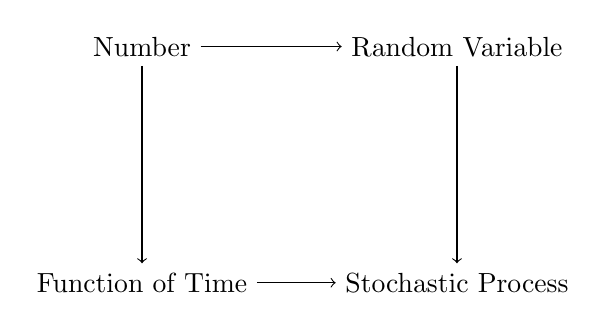
\begin{tikzpicture}
        \draw (0, 3) node[](num){Number};
        \draw (0, 0) node[](fot){Function of Time};
        \draw (4, 0) node[](sto){Stochastic Process};
        \draw (4, 3) node[](rv){Random Variable};
        \draw[->] (num) -- (rv);
        \draw[->] (num) -- (fot);
        \draw[->] (fot) -- (sto);
        \draw[->] (rv) -- (sto);
    \end{tikzpicture}
\end{center}
Therefore the two interpretations of a stochastic process are as follows:
\begin{enumerate}
    \item A sequence of random variables
    \item A random function
\end{enumerate}
Attempts to formulate the second interpretation have faced many difficulties. As such, we define a stochastic process as:
\section{DTMC}

\subsection{Review of Probability}

A \term{random variable (r.v.)}  $X$ is a real valued function of the outcomes of a random experiment.

\[ X : \Om \to R \]

Where $\Om = \bc{\w_1, \w_2, \ldots}$ is the \term{sample space} corresponding to all possible outcomes $\w_i$. The outcomes can in principle be any objects (numbers, strings, etc.). We say that $X$ maps each outcome $\w$ to a real number $\w \mapsto X\br{\w} \in \R$. \\

A \term{stochastic process} is a family of random variables $\bc{X_t}_{t \in T}$, defined on a common sample space $\Om$. $T$ is referred to as the index set for the stochastic process which is often understood as time. The index set $T$ can take a discrete spectrum,
\[ T = \bc{0, 1, 2, \ldots} \qquad \bc{X_n \mid n = 0, 1, 2, \ldots} \]
Alternatively, $T$ can take on a continuous spectrum,
\[ T = \bc{t \mid t \geq 0} = \left[ 0 , \inf \right) \]

The \term{state space} $S$ is the collection of all possible values of $X_t$'s. It is important to understand the distinction of between sample space and state space. Additionally, the state space can either have discrete or continuous spectrum. \\

A question remains, \textit{Why do we need the family of random variables to be defined on a common sample space?} The answer being that we would like to be able to discuss the joint behaviour of $X_t$'s. If $X_1$ has domain $\Om_1$ and $X_2$ has domain $\Om_2$ (where $\Om_1 \neq \Om_2$), then one can \textit{not} talk about common ideas of correlations and associations between $X_1$ and $X_2$. As such we assert that all members of a stochastic process share the same sample space domain $\Om$.

\subsection{Discrete-time Markov Chain}

A \term{discrete-time stochastic process} $\bc{X_n \mid n \in 0, 1, 2, \ldots}$ is said to be a \term{Discrete-time Markov Chain (DTMC)}  if the following conditions hold:
\begin{enumerate}
    \item The state space is at most \textit{countable}\footnote{Countable meaning there is a one-to-one mapping from the state space to the natural numbers.} (i.e. finite or countable).
    \[ S = \bc{0, 1, \ldots, k} \quad \textrm{or} \quad S = \bc{0, 1, 2, \ldots} \]
    \item \term{Markov Property}: For any $n = 0, 1, 2, \ldots$,
    \[ P\br{X_{n+1} = x_{n+1} \mid X_n = x_n, X_{n-1} = x_{n-1}, \ldots, X_{0} = x_{0}} = P\br{X_{n+1} = x_{n+1} \mid X_{n} = x_{n}} \]
\end{enumerate}
We use capital letters $X$ to denote the random variable and lower case letters $x$ to denote a specific realization or valuation of $X$. The motivation of the Markov property is that future events $X_{n+1} = x_{n+1}$ are independent of past histories $\bc{X_{i} = x_{i} \mid i = 0, 1, \ldots, n-1}$ given the immediate past state $X_{n} = x_{n}$. The intuition being that the future and the past are probabilistically independent.

\begin{center}
    \textit{Given the present, the future and the past are independent.}
\end{center}

% === Notes for GONGCHEN ===
\subsection{Transition Probability}

The \term{transition probability} from a state $i \in S$ at time $n$ to state $j \in S$ (at time $n+1$) is given by,
\[ P_{n, i, j} \defined P \br{X_{n+1}= j \mid X_{n} = i} \qquad n = 0, 1, 2, \ldots \eq \label{eq:trans_prob}\]
In full generality, the transition probability could depend on time $n$ but in this course we will restrict ourselves to transition probabilities that \textit{do not} depend on time $n$ ($P_{n, i, j} = P_{i, j}$). We say that the markov chain is \term{(time-)homogeneous} if this property holds. From now on, this will be our default setting. \\

The matrix of all transition probabilities $P = \bc{P_{i,j} \mid i,j \in S}$ is called the \term{one-step transition (probability) matrix} for $\bc{X_{n} \mid n \in T}$.
\[ P = \begin{pmatrix}
P_{00} & P_{01} & \cdots & P_{0j} & \cdots \\
P_{10} & P_{11} & \cdots & P_{1j} & \cdots \\
\vdots & \vdots & \ddots & \vdots & \cdots \\
P_{i0} & P_{i1} & \cdots & P_{ij} & \cdots \\
\vdots & \vdots & \vdots & \vdots & \ddots
\end{pmatrix} \]
The one-step transition matrix $P$ has the following properties:
\begin{enumerate}
    \item The entries of $P$ are non-negative:
    \[ P_{i,j} \geq 0 \eq \label{eq:trans_positive_entries} \]
    \item The rows of $P$ sum to unity:
    \[ \forall i : \sum_{j \in S} P_{ij} = 1 \eq \label{eq:trans_row_sum} \]
\end{enumerate}

The \term{n-step transition probability} is defined via the homogeneous property,
\[ \forall i,j \in S : P_{ij}^{(n)} \defined P\br{X_{n+m} = j \mid X_{n} = i} = P\br{X_{n} = j \mid X_{m} = i} \]
Analogously, the \term{n-step transition matrix} is the matrix,
\[ P^{(n)} = \bc{P_{ij}^{(n)} \mid i, j \in S} \]

\begin{theorem}
There is a simple relation between the n-step transition matrix $P^{(n)}$ and the one step transition matrix $P$.
\[ P^{(n)} = P^{(n-1)} \cdot P = \underbrace{P \cdot P \cdot \cdots \cdot P}_{n} = P^n \]
\end{theorem}

\begin{proof}
Proof by induction:
\[ P^{(1)} = P \note{By definition.} \]
We also have $P^{(0)} = P^{0} = \ind$ is the identity matrix. We now assume $P^{(n)} = P^{n}$. Then $\forall i,j \in S$,
\begin{align*}
    P_{ij}^{(n+1)} &= P\br{X_{n+1} = j \mid X_{0} = i} \\
    &= \sum_{k \in S} P\br{X_{n+1} = j, X_{n} = k \mid X_{0} = i} \note{Total probability}\\
    &= \sum_{k \in S} \f{P\br{X_{n+1} = j, X_{n} = k, X_{0} = i}}{P\br{X_{0} = i}} \\
    &= \sum_{k \in S} \f{P\br{X_{n+1} = j, X_{n} = k, X_{0} = i}}{P\br{X_{n} = k, X_{0} = i}}\f{P\br{X_{n} = k, X_{0} = i}}{P\br{X_{0} = i}} \\
    &= \sum_{k \in S} P\br{X_{n+1} = j \mid X_{n} = k, X_{0} = i} \cdot P\br{X_{n} = k \mid X_{0} = i} \note{Conditional total probability}\\
    &= \sum_{k \in S} P\br{X_{n+1} = j \mid X_{n} = k} \cdot P\br{X_{n} = k \mid X_{0} = i} \note{Use Markov Property}\\
    &= \sum_{k \in S} P_{kj} \cdot P_{ik}^{(n)} \note{Matrix terms}\\
    &= \br{P \cdot P^{(n)}}_{ij} \note{Matrix product}\\
    &= \br{P^{n+1}}_{ij} \note{Inductive Hypothesis}
\end{align*}
There we have proved that $P^{(n+1)} = P^{n+1}$ and so we have a completed the proof that $P^{(n)} = P^{n}$.\\
\end{proof}

This result is very fundamental. We now have a relationship between the $n$-step transition matrix and the $1$-step transition matrix (namely $P^{(n)} = P^n$). It is important to not to be confused by notation ($P^{(n)} = P^n$ is not a tautology). $P^{(n)}$ is a single matrix with entries populated by $n$-step transition probabilities while $P^n$ is a single matrix multiplied by itself $n-1$ times.

\begin{corollary}
As a corollary, we have obtained that,
\[ P^{(n)} = P^{(m)} \cdot P^{(n-m)} \quad \forall 0 \leq m \leq n \]
Or equivalently the \textbf{Chapman-Kolmogorov (C-K) Equation},
\[ P^{(n)}_{ij} = \sum_{k \in S} P^{(m)}_{ik} P^{(n-m)}_{kj} \quad \forall i,j \in S, \forall 0 \leq m \leq n \eq \label{eq:ck_equation} \]
\end{corollary}

It is very common to use the entry-wise form of the C-K equation (\cref{eq:ck_equation}) instead of the more compact but less expressive matrix form ($P^{(n)} = P^{(m)} \cdot P^{(n-m)}$). Pictorially the C-K gives reveals the following picture that holds for all Markov chains,

\begin{center}
    \begin{tikzpicture}
    \begin{scope}
        \tikzstyle{every node}=[fill=black, draw=black, circle, inner sep=1.2pt]
        \node[label=left:$i$] (i) at (0,0) {};
        \node[label=right:$j$] (j) at (4,0) {};
        \node[label=above right:$0$] (k0) at (2,2) {};
        \node[label=above right:$1$] (k1) at (2,1) {};
        \node[label=above:$k-1$] (kkm1) at (2,-1) {};
        \node[label=below right:$k$] (kk) at (2,-2) {};
    \end{scope}
    \begin{scope}[decoration={markings, mark=at position 0.5 with {\arrow{>}}}]
        \draw[postaction={decorate}] (i) -- node[above left]{$P^{(m)}_{i0}$} (k0);
        \draw[postaction={decorate}] (i) -- (k1);
        \draw[postaction={decorate}] (i) -- (kkm1);
        \draw[postaction={decorate}] (k0) -- node[above right]{$P^{(n)}_{0j}$} (j);
        \draw[postaction={decorate}] (k1) -- (j);
        \draw[postaction={decorate}] (kkm1) -- (j);

        \draw[postaction={decorate}] (i) -- node[below left]{$P^{(m)}_{ik}$}(kk);
        \draw[postaction={decorate}] (kk) -- node[below right]{$P^{(n)}_{kj}$} (j);
    \end{scope}
    \draw[dashed] (2, 2.5) -- (2, -2.5);
    \draw[dashed] (0, 2.5) -- (0, -2.5);
    \draw[dashed] (4, 2.5) -- (4, -2.5);
    \draw[] (2, 2.5) node[above]{$m$};
    \draw[] (4, 2.5) node[above]{$m+n$};
    \draw[] (0, 2.5) node[above]{$0$};
    \end{tikzpicture}
\end{center}

So far, we have only been discussing transition probabilities. We will now divert our attention to actual distributions for a stochastic process. \\

Let $\al_n = \br{\al_{n, 0}, \al_{n, 1}, \ldots}$ be the \term{probability distribution vector} for $X_n$ at time $n$.
\[ \al_{n,k} = P\br{X_n = k} \qquad \forall k \in S \]
Note that $\al_{n,k} \geq 0$ and $\sum_{k\in S} \al_{n, k} = 1$ and $n = 0, 1, 2,\ldots$. We also define the initial distribution $\al_0$,
\[ \al_0 = \br{P\br{X_0 = 0}, P\br{X_0 = 1}, \ldots} \]
\begin{theorem}
The transition probability matrix reveals the following relationship between the distribution $\al_n$ at time $n$ and the distribution $\al_0$ at time $0$,
\[ \al_n = \al_0 \cdot P^{n} \eq \label{eq:transition_dist}\]
\end{theorem}
\begin{proof}
The proof \cref{eq:transition_dist} is quite trivial:
\begin{align*}
    \forall j \in S \quad \al_{n, j} &= P\br{X_n = j} \\
     &= \sum_{i \in S} P\br{X_n = j \mid X_0 = i} \cdot P\br{X_0 = i} \\
     &= \sum_{i \in S} \al_{0, i} \cdot P_{ij}^{n} \\
     &= \al_{0, 0} \cdot P_{0j}^{n} + \al_{0, 1} \cdot P_{1j}^{n} + \ldots \\
     &= \br{\al_{0} \cdot P^{n}}_j
\end{align*}
\end{proof}
More generally, for any $n = 1, 2, \ldots$ the finite dimensional distribution can be obtained from the following process iterative process,
\begin{align*}
&\hspace{-0.5in}P\br{X_n=x_n, X_{n-1}=x_{n-1}, \ldots, X_{0}=x_{0}} = \\
&P\br{X_{0} = x_{0}} \cdot\\
&P\br{X_{1} = x_{1} \mid X_0 = x_0} \cdot\\
&P\br{\val{2} \mid \val{1}, \val{0}} \cdots \\
&P\br{\val{n} \mid \val{n-1}, \ldots, \val{0}}
\end{align*}
But by the Markov condition, it must be that,
\begin{align*}
&\hspace{-0.5in}P\br{X_n=x_n, X_{n-1}=x_{n-1}, \ldots, X_{0}=x_{0}} = \\
&P\br{X_{0} = x_{0}} \cdot\\
&P\br{X_{1} = x_{1} \mid X_0 = x_0} \cdot \\
&P\br{\val{2} \mid \val{1}} \cdots \\
&P\br{\val{n} \mid \val{n-1}}
\end{align*}
First recognize the first term on the RHS ($P\br{X_{0} = x_{0}} = \al_{0, x_0}$), and also the remaining terms are transition probabilities as per \cref{eq:trans_prob}. Therefore it must be that,
\[ P\br{X_n=x_n, X_{n-1}=x_{n-1}, \ldots, X_{0}=x_{0}} = \al_{0, x_0} P_{x_0x_1}P_{x_1x_2}\cdots P_{x_{n-1}x_n} \]
Even more generally, for $0 \leq t_1 < t_2 < \cdots < t_n$,
\[ P\br{\val{t_n}, \val{t_{n-1}}, \ldots, \val{t_{1}}} = P\br{\val{t_1}} \br{P^{t_2 - t_1}}_{x_{t_1}x_{t_2}}\br{P^{t_3 - t_2}}_{x_{t_2}x_{t_3}}\cdots\br{P^{t_{n} - t_{n-1}}}_{x_{t_{n-1}}x_{t_{n}}}  \]
Since $P\br{\val{t_1}} = \al_{t_1 x_{t_1}} = \sum_{k \in S} \al_{0, k} P^{t_1}_{k, x_{t_1}}$,
\[ \al_{t_1} = \al_{0} \cdot P^{t_1} \eq \label{eq:distribution_fundamentals} \]
\begin{remark}
\Cref{eq:transition_dist} carries a very important interpretation. The probabilistic properties of a Discrete-Time Markov Chain (DTMC) are fully characterized by two things:
\begin{enumerate}
    \item The initial distribution $\al_{0}$
    \item Transition matrix $P$
\end{enumerate}
Knowing both the initial distribution and transition matrix fully determines the distribution $\al_{n}$ for all times $n$.
\end{remark}

\subsection{Stationary Distribution (Invariant Distribution)}
In this section, we are interested in determining which distributions $\al_{0}$ remain unchanged for all time $n \in T$.
\begin{definition}
    A probability distribution $\pi = \br{\pi_0, \pi_1, \cdots}$ is called a \term{stationary (invariant) distribution} of the DTMC $\bc{X_n}_{n = 0,1, \cdots}$ with transition matrix $P$ if the following conditions hold,
    \begin{enumerate}
        \item The transition matrix does not change $\pi$:
        \[  \pi = \pi \cdot P \eq \label{eq:invariant}\]
        \item The vector $\pi$ is a valid probability distribution,
        \[ \sum_{i \in S} \pi_i = 1 \qquad \pi_i \geq 0 \eq \label{eq:prob_dist_requirements}\]
    \end{enumerate}
\end{definition}
Notice that if we posit that $\pi$ is a probability distribution, then the second condition is already satisfied. Nonetheless, in practice we are able to find candidate $\pi$'s using the the first condition and then we need to check these candidates against the second condition. In general, if $\sum_{i \in S} \pi_i$ is bounded (i.e. $\sum_{i \in S} \pi_i < \inf$) then it is possible to normalize the candidate $\pi$ in order to satisfy \cref{eq:prob_dist_requirements}. \\

\textit{Why are such $\pi$'s called stationary/invariant distributions?} Notice that \cref{eq:invariant} completely answers this question. Assume that the MC starts with initial distribution $\al_0 = \pi$ for $X_0$. In this case, the distribution of $X_1$ is determined by $P$,
\[ \al_1 = \al_0 \cdot P \]
But since $\al_0$ is $\pi$ and $\pi$ satisfies \cref{eq:invariant},
\[ \al_1 = \pi \cdot P = \pi \]
The distribution for $X_1$ is the \textit{same} as the distribution for $X_0$. This process continues,
\[ \al_2 = \al_1 \cdot P = \pi \cdot P = \pi \]
\[ \al_n = \al_0 \cdot P^n = \pi \cdot P^n = \pi \cdot P^{n-1} = \cdots = \pi \]
Thus if the Markov chain starts with a stationary/invariant distribution then its marginal distribution will \textit{never change}; hence why we refer $\pi$ as stationary. Also not that this \textit{does not} indicate that the value of $X_i$ does not change over time (it almost certainly will), but its distribution does.

\begin{example}
    Consider an electron with two states: ground $(0)$ and excited $(1)$. Let $X_n$ be the state at time $n$. At each step, with probability $\al$ the MC chains state if it is in the ground state. With probability $\be$ the MC will transition to the ground state if it is in the excited state. Then $\bc{X_n}_{n=0,1,\ldots}$ is a DTMC and its transition matrix is,
    \[ P = \kbordermatrix{
         & (0) & (1) \\
        (0) & 1 - \al & \al \\
        (1) & \be & 1 - \be \\
    } \]
    Now let us solve for the stationary distribution $\pi$.
    \[ \pi = \pi \cdot P \qquad \pi = \br{\pi_0, \pi_1} \qquad \pi_0 + \pi_1 = 1 \]
    Therefore,
    \begin{align*}
    \pi_0 &= \br{1 - \al} \pi_0 + \be \pi_1 \eq \label{eq:qe1}\\
    \pi_1 &= \al \pi_0 + \br{1 - \be} \pi_1 \eq \label{eq:qe2}
    \end{align*}
    However note that these two equations are not linearly independent. This is evident because summing \cref{eq:qe1} with \cref{eq:qe2} results in the trivial statement of $\pi_0 + \pi_1 = \pi_0 + \pi_1$. Nonetheless rearranging \cref{eq:qe1} gives,
    \[ \al \pi_0 = \be \pi_1 \implies \f{\pi_0}{\pi_1} = \f{\be}{\al} \]
    This is where we need $\pi_0 + \pi_1 = 1$.
    \[ \pi_0 = \f{\be}{\al+\be} \qquad \pi_1 = \f{\al}{\al+\be} \]
    Where $\al + \be$ is considered the normalizing constant.
\end{example}

An important remark: sometimes the candidate distribution is not normalizable. In particular, there are configurations where \cref{eq:invariant} is satisfiable but \cref{eq:prob_dist_requirements} is not. In the above example, there exists a unique stationary distribution,
\[ \pi = \br{\f{\al}{\al + \be} ,\f{\be}{\al + \be}} \]
If $\al_0 = \pi$ then we know immediately that,
\[ P\br{X_n = 0} = \f{\be}{\al+\be} \qquad P\br{X_n = 1} = \f{\al}{\al+\be} \qquad \forall n = 1, 2, \ldots\]
\begin{remark}
    By the above procedure of solving for stationary distribution is typical.
    \begin{enumerate}
        \item Use \cref{eq:invariant} to get proportions between different components of $\pi$.
        \item Use \cref{eq:prob_dist_requirements} to normalize $\pi$ and get exact values.
    \end{enumerate}
\end{remark}
\begin{remark}
    Note that if $\be = 2 \al$ then $\pi$ is always $\br{2/3, 1/3}$ regardless the actual value of $\al$.
\end{remark}
% === Notes for GONGCHEN ===
% === CONTINUE ===

\subsection{Classification of States}
\newcommand{\comm}{\leftrightarrow}
\newcommand{\acc}[2]{#1 \to #2}

State $j$ is \term{accessible} from state $i$ (denoted $\acc{i}{j}$) if there exists $n = 0, 1, \ldots$ such that $P^{(n)}_{ij} > 0$. Intuitively, one can transition from state $i$ to state $j$ in finite steps $n$ with positive probability. If $i$ is also accessible from $j$, then we say $i$ and $j$ \term{communicate}, denoted as ${i}\comm{j}$.
\[ {i}\comm{j} \Leftrightarrow \exists m, n \geq 0, P_{ij}^{(m)} > 0, P_{ji}^{(n)} > 0 \]
\begin{theorem}
The binary communication relation ``${}{\comm}$'' is in fact a equivalence relation:
\begin{itemize}
    \item Reflexivity ${i}\comm{i}$
    \item Symmetry ${i}\comm{j} \implies {j}\comm{i}$
    \item Transitivity ${i}\comm{j}, {j}\comm{k} \implies {i}\comm{k}$
\end{itemize}
\end{theorem}
\begin{proof}
First, reflexivity is easy to prove by definition. Let $n = 0$ and recognize that $P^{(0)}_{ii}$ has a certain probability by definition,
\[ P^{(0)}_{ii} = 1 \implies {i}\comm{i} \]
Second, symmetry follows by definition,
\[ P_{ij}^{(m)} > 0, P_{ji}^{(n)} > 0 \Leftrightarrow P_{ji}^{(n)} > 0, P_{ij}^{(m)} > 0 \]
Third, transitivity can be proving by letting $m$ and $n$ be the unknown quantifiers:
\[ \exists m \quad P_{ij}^{(m)} > 0, \exists n \quad P_{jk}^{(n)} > 0 \]
Then by the CK equation \cref{eq:ck_equation},
\[ P^{(m+n)}_{ik} = \sum_{l \in S} P^{(m)}_{il}P^{(n)}_{lk} \]
Let $l = j$ be a single, fixed entry in the summation,
\[ P^{(m+n)}_{ik} \geq P^{(m)}_{ij}P^{(n)}_{jk} > 0 \]
Therefore we have that $k$ is accessible from $i$ ($\acc{i}{j}$). Analogously we have that $\acc{i}{j}$ therefore ${i}\comm{k}$. \\
\end{proof}
The communication equivalence relations then divides the state space $S$ into different equivalence classes. That is, the states in one class comm with each other; the states in different classes do not comm. The equivalent classes form a \textit{partition} of the state space $S$. \\

The family $\bc{S_1, S_2, \ldots S_n}$ is a \term{partition} of $S$ if,
\begin{enumerate}
    \item $S_i \subset S \mid \forall i \in 1,2,\ldots,n$
    \item $S_i \cap S_j \neq \emptyset$ for all $i \neq j$
    \item $\bigcup_{i} S_i = S$
\end{enumerate}

We can find the equivalent classes by drawing a graph where the states in $S$ are the nodes of the graph and a directed edge is placed going from $i$ to $j$ if $j$ is accessible from $i$ in one-step: $P_{ij} > 0$. Then identifying the the equivalent classes corresponds to identifying the loops of this graph within one step. \\


\begin{example}

As an example, consider the transition matrix $P$ as follows.

\[ P = \kbordermatrix{
    & 0 & 1 & 2 & 3 & 4 \\
    0& 0.2 & 0.8 & 0 & 0 & 0 \\
    1& 0.6 & 0.4 & 0 & 0 & 0 \\
    2& 0 & 0.5 & 0 & 0.5 & 0 \\
    3& 0 & 0 & 0 & 0.7 & 0.3 \\
    4& 0 & 0 & 0 & 0.1 & 0.9} \]

The associated one-step accessibility graph is then,
\begin{center}
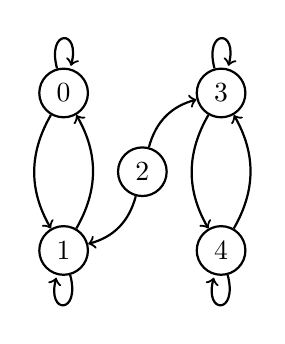
\begin{tikzpicture}
    \begin{scope}
        \tikzstyle{every node}=[fill=white, draw=black, circle, thick, text=black, scale=1.0]
        \node (0) at (0,2) {$0$};
        \node (1) at (0,0) {$1$};
        \node (2) at (1,1) {$2$};
        \node (3) at (2,2) {$3$};
        \node (4) at (2,0) {$4$};
    \end{scope}
    \begin{scope}
        \tikzstyle{every edge}=[draw, thick, ->]
        \path
        (0) edge[bend right] (1)
        (1) edge[bend right] (0)
        (0) edge[loop above] (0)
        (1) edge[loop below] (1)
        (3) edge[bend right] (4)
        (4) edge[bend right] (3)
        (3) edge[loop above] (3)
        (4) edge[loop below] (4)
        (2) edge[bend left] (3)
        (2) edge[bend left] (1);
    \end{scope}
\end{tikzpicture}
\end{center}

Where the loops of $S = \bc{0,1,2,3,4}$ form the following partition,
\[ S_1 = \bc{0,1} \quad S_2 = \bc{2} \quad S_3 = \bc{3, 4} \]
\end{example}

These equivalent classes are useful for Markov chains because it allows one to separate the behaviour of the equivalence classes and study them individually. A MC which has only one equivalent class is called \term{irreducible}. \\

\begin{example}
    \[ P = \kbordermatrix{
          & 0 & 1 & 2 & 3 \\
        0 & 0 & 1 & 0 & 0 \\
        1 & 0.5 & 0 & 0.5 & 0 \\
        2 & 0 & 0.5 & 0 & 0.5 \\
        3 & 0 & 0 & 1 & 0 \\
    } \]
    \begin{center}
    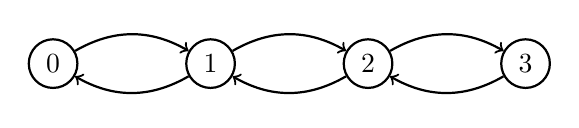
\begin{tikzpicture}
        \begin{scope}
            \tikzstyle{every node}=[fill=white, draw=black, circle, thick, text=black, scale=1.0]
            \node (0) at (0,0) {$0$};
            \node (1) at (2,0) {$1$};
            \node (2) at (4,0) {$2$};
            \node (3) at (6,0) {$3$};
        \end{scope}
        \begin{scope}
            \tikzstyle{every edge}=[draw, thick, ->]
            \path
            (0) edge[bend left] (1)
            (1) edge[bend left] (2)
            (2) edge[bend left] (3)
            (3) edge[bend left] (2)
            (2) edge[bend left] (1)
            (1) edge[bend left] (0)
            ;
        \end{scope}
    \end{tikzpicture}
    \end{center}
    Clearly if we start at state $0$, we can only go back to $0$ in $2,4,6,\ldots$ (i.e. an even number of) steps.
\end{example}
Furthermore, let us define the \term{period} of state $i$ as,

\[ d\br{i} = \gcd \bc{n \in \Z^{+} \mid P_{ii}^{n} > 0} \]

Additionally, if $P_{ii}^{n} = 0$ holds for all $n > 0$, we say that $d\br{i} = \inf$. If the period of $i$ happens to be $d\br{i} = 1$ then the state $i$ is said to be \term{aperiodic}. Alternatively, locus of steps that we can go back by are \textit{co-prime}. A MC is called aperiodic if all its states $S$ are aperiodic.\\

Note that $P_{ii} < 0$ then the greatest common divisor must be one. This implies that $d_i = 1$. In this case, the state is immediately aperiodic.\\

The period of a state is useful do to the following theorem,

\begin{theorem}
\label{thm:period_class_prop}
The period of a state is a class property. If ${i}\comm{j}$, then $d\br{i} = d\br{j}$.
\end{theorem}

\begin{proof}
If $i = j$ we are already done. If $i \neq j$, since ${i}\comm{j}$, then $\exists n, m$ such that,
\[ P_{ij}^{n} > 0 \quad P_{ji}^{m} > 0 \]
Then for any $l$ such that $P^{l}_{jj} > 0$,
\[ P_{ii}^{n+m+l} \geq P_{ij}^{n}P_{jj}^{l}P_{ji}^{m} \eq \label{eq:period_class_prop_2} \]
Because $P_{ij}^{n}P_{jj}^{l}P_{ji}^{m}$ happens to be a specific way for $P_{ii}^{n+m+l}$ to occur. Since ${i}\comm{j}$ and $l$ was chosen carefully,
\[ P_{ii}^{n+m+l} > 0 \]
Moreover, we also have that,
\[ P_{ii}^{n+m} \geq P_{ij}^{n}P_{ji}^{m} \eq \label{eq:period_class_prop_1}\]
Since $d\br{i}$ divides both $n+m$ and $n+m+l$ by \cref{eq:period_class_prop_1,eq:period_class_prop_2}, then $d\br{i}$ also divides $l$. This holds for all $l$ such that $P_{ii}^{l}>0$. This implies that $d\br{i}$ is a common divisor of $\bc{l \mid P_{jj}^{l} > 0}$ an thus $d\br{i}$ divides,
\[ d\br{j} = \gcd \bc{l \mid P_{jj}^{l} > 0} \]
By symmetry $d\br{j}$ divides $d\br{i}$. Therefore $d\br{i} = d\br{j}$. \\
\end{proof}

\begin{remark}
It is important to note that $d\br{i} = k \not\Rightarrow P_{ii}^{(k)} > 0$. As a counterexample consider the following one step accessibility graph,
\begin{center}
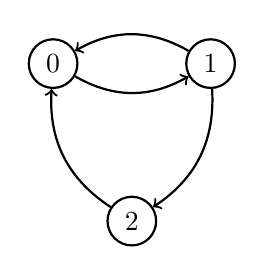
\begin{tikzpicture}
    \begin{scope}
        \tikzstyle{every node}=[fill=white, draw=black, circle, thick, text=black, scale=1.0]
        \node (0) at (-1,2) {$0$};
        \node (1) at (1,2) {$1$};
        \node (2) at (0,0) {$2$};
    \end{scope}
    \begin{scope}
        \tikzstyle{every edge}=[draw, thick, ->]
        \path
        (0) edge[bend right] (1)
        (1) edge[bend right] (0)
        (2) edge[bend left] (0)
        (1) edge[bend left] (2);
    \end{scope}
\end{tikzpicture}
\end{center}
Evidently,
\[ P^{(2)}_{00} > 0 \quad P^{(3)}_{00} > 0 \]
So we have $d\br{0} = 1$ because $d\br{0} = \gcd\bc{2,3,\ldots}$. However this doesn't imply that $P_{00}^{(1)} > 0$ because we do have that $P^{(1)}_{00} = 0$
\end{remark}

\begin{remark}
If the MC is irreducible (having only one class) then all the states have the same period. In this case we ascribe the entire MC the period $d\br{i}$ for some representative $ i \in S$.
\end{remark}

\begin{remark}
    If the period of $i$ is $d_i = 1$ then there exists some $N$ such that $P_{ii}^{(n)} > 0$ for any $n \geq N$. Intuitively, if state $i$ is aperiodic then after a long time, the probability of going back to $i$ is always positive.
\end{remark}

\subsection{Recurrence and Transience}
In order to define transience and recurrence, let $T_i$ be the waiting time of a MC to visit/revisit state $i$ for the first time since time $0$.
\[ T_i = \min \bc{n > 0 : X_n = i} \]
Of course we have that $\bc{n > 0 : X_n = i}$ is a random collection of numbers and also $\min\bc{n > 0 : X_n = i}$ is a random number. Therefore $T_i$ is a random variable. Notice that if $T_i = \inf$ if the MC never returns to state $i$.
\begin{definition}
    A state $i$ is called \term{transient} if,
    \[ P\br{T_i < \inf \mid X_0 = i} < 1 \]
    Or equivalently,
    \[ P\br{T_i = \inf \mid X_0 = i} > 0 \]
    We say that the MC never goes back to state $i$ with positive probability.
\end{definition}
Moreover,
\begin{definition}
    A state $i$ is \term{recurrent} if,
    \[ P\br{T_i < \inf \mid X_0 = i} = 1 \]
    Or equivalently,
    \[ P\br{T_i = \inf \mid X_0 = i} = 0 \]
    We say that the MC always goes back to $i$.
\end{definition}
\begin{remark}
    If we have that $P\br{T < \inf} = 1$ then it does not imply that $\Exp\br{T} < \inf$. As a counter example, let $s_p = 2^{p}$ for $p = 1, \ldots, \inf$,
    \[ P\br{T = s_p} = \f{1}{s_p} \]
    Where the expectation of $T$ is unbounded,
    \[ \Exp\br{T} = \sum_{p=1}^{\inf} s_p \f{1}{s_p} = \sum_{p=1}^{\inf} 1 = \inf \]
\end{remark}
To make the distinction,
\begin{definition}
    A recurrent state $i$ is said to be \term{positive recurrent} if,
    \[ \Exp\br{T_i \mid X_0 = i} < \inf \]
    A recurrent state $i$ is said to be \term{null recurrent} if,
    \[ \Exp\br{T_i \mid X_0 = i} = \inf \]
\end{definition}

\begin{example}
    Consider the following example with transition matrix,
    \[ P \kbordermatrix{
          & 0 & 1 & 2 \\
        0 & \f12 & \f12 & 0 \\
        1 & 0 & \f12 & \f12 \\
        2 & 0 & 0 & 1 \\
    } \]
    And MC graphically expressed as,
    \begin{center}
    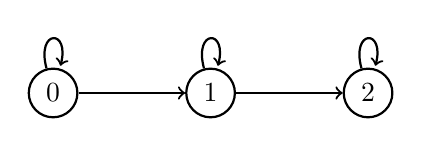
\begin{tikzpicture}
        \begin{scope}
            \tikzstyle{every node}=[fill=white, draw=black, circle, thick, text=black, scale=1.0]
            \node (0) at (0,0) {$0$};
            \node (1) at (2,0) {$1$};
            \node (2) at (4,0) {$2$};
        \end{scope}
        \begin{scope}
            \tikzstyle{every edge}=[draw, thick, ->]
            \path
            (0) edge[] (1)
            (1) edge[] (2)
            (0) edge[loop above] (0)
            (1) edge[loop above] (1)
            (2) edge[loop above] (2);
        \end{scope}
    \end{tikzpicture}
    \end{center}
    Given that $X_0 = 0$ there are only two possibilities for transitions,
    \[ P\br{\underbrace{X_1 = 0 \mid X_0 = 0}_{T_0 = 1}} = P\br{\underbrace{X_1 = 1 \mid X_0 = 0}_{T_0 = \inf}} = \f12 \]
    The second term is recognized as $T_0 = \inf$ because after transitioning to state $1$, it is impossible to return to state $0$. This tells us that,
    \[ P\br{T_0 < \inf \mid X_0 = 0} = \f{1}{2} < 1 \]
    Therefore state $0$ is said to be transient. Analogously we have that state $1$ is also transient. Given $X_0 = 2$, $P\br{\underbrace{X_1 = 2 \mid X_0 = 2}_{T_2=1}} = 1$ we have that,
    \[ P\br{T_2 < \inf \mid X_0 = 2} - 1 \]
    Which tells is that state $2$ is recurrent.
\end{example}
In general, the distribution of $T_i$ is very hard to derive. In particular it will be hard to know whether $T_i$ takes value $\inf$ and with what probability. This suggests that we will need handier criteria for recurrence/transience. \\

To facilitate this define $f_{ii} = P\br{T_i < \inf \mid X_0 = i}$ and,
\[ f_{ij} = P\br{T_j < \inf \mid X_0 = i} \]
We also defined $V_i$ to be the number of times that the MC visits state $i$,
\[ V_i = \sum_{n=1}^{\inf} \ident_{\bc{X_n = i}} \]
First consider the case that $i$ is transient. If $i$ is transient, then it must be that $f_{ii} < 1$. This can be seen from the definition of $T_i$. The PMF is,
\[ P\br{V_i = k \mid X_0 = i} = f_{ii}^{k} \br{1 - f_{ii}} \]
This can be derived by considering that if the MC is to visit state $i$ exactly $k$ times but not more than $k$ times.
\[ P\br{V_i = k \mid X_0 = i} = \bs{P\br{T_i < \inf \mid X_0 = i}}^{k} \bs{P\br{T_i = \inf \mid X_0 = i}} \]
This PMF tells us that $V_i + 1$ follows a geometric distribution with parameter $1 - f_{ii}$,
\[ V_i + 1 \sim \Geo\br{1 - f_{ii}} \]
In particular, $P\br{V_i < \inf \mid X_0 = i} = 1$. Therefore if $i$ is transient, it is visited only finitely many times with probability $1$. Afterwards, the MC will leave state $i$ forever sooner or later.\\

Second consider the case that $i$ is recurrent. If state $i$ is recurrent, then $f_{ii} = 1$ by definition. The we have that,
\[P\br{V_i = k\mid X_0 = i} = 0 \quad \forall k = 0, 1, \ldots  \]
Since $V_i$ can not take on any finite values, it must be that
\[ P\br{V_i = \inf\mid X_0 = i} = 1 \]
If the MC starts from recurrent state $i$ is will visit that state infinitely many times. Before identifying our more versatile criteria, we generalize some of these notions.
\subsection{Recurrence and Transience Again}
For $n \in \Z^{+}$ define,
\[ f_{ij}^{(n)} = P \br{X_n = j, X_{n-1} \neq j, \cdots, X_{1} \neq j \mid X_0 = i} \quad \forall i,j \in S \]
Intuitively, $f_{ij}^{(n)}$ is the probability that $X$ visits state $j$ at time $n$ for the first time since $X_0 = i$. A looming question: What is the relation between $f_{ij}^{(n)}$ and $P_{ij}^{(n)}$? First notice that,
\[ P_{ij}^{(n)} \geq f_{ij}^{(n)} \]
These reads: the probability that $X$ visits $j$ at time $n$ is more larger that the probability that $X$ visits $j$ at time $n$ provided it did not visit $j$ prior. A more detailed equality is the following,
\[ P_{ij}^{(n)} = \sum_{k = 1}^{n} f_{ij}^{(k)}P_{jj}^{(n-k)} \eq \label{eq:recurrence_form}\]
Expanded out gives,
\[ P_{ij}^{(n)} = f_{ij}^{(n)} + \sum_{k = 1}^{n-1} f_{ij}^{(k)}P_{jj}^{(n-k)} \]
\begin{proof}
\begin{align*}
P_{ij}^{(n)} & = P\br{X_n = j \mid X_0 = i} \\
& = \sum_{k=1}^{n} P\br{X_n = j, \text{$X$ first visits $j$ at time $k$} \mid X_0 = i} \\
& = \sum_{k=1}^{n} P\br{X_n = j, \mid \text{$X$ first visits $j$ at time $k$}, X_0 = i} \cdot P\br{\text{$X$ first visits $j$ at time $k$} \mid X_0 = i} \\
& = \sum_{k=1}^{n} P\br{X_n = j, \mid X_k = j, X_{k-1} \neq j, \ldots, X_{1} \neq j, X_0 = i} \cdot P\br{X_k = j, X_{k-1} \neq j, \ldots, X_{1} \neq j \mid X_0 = i} \\
& = \sum_{k=1}^{n} P\br{X_n = j, \mid X_k = j, X_{k-1} \neq j, \ldots, X_{1} \neq j, X_0 = i} \cdot f_{ij}^{(k)} \\
& = \sum_{k=1}^{n} P\br{X_n = j, \mid X_k = j} \cdot f_{ij}^{(k)} \note{Markov Condition} \\
& = \sum_{k=1}^{n} P^{(n-k)}_{jj} \cdot f_{ij}^{(k)}
\end{align*}
\end{proof}
In fact \cref{eq:recurrence_form} defines a recurrence relation to compute $f_{ij}^{(n)}$ from $f_{ij}^{(k)}$ where $k < n$,
\[ f_{ij}^{(n)} = P_{ij}^{(n)} - \sum_{k=1}^{n-1} f_{ij}^{(k)} P_{jj}^{(n+k)} \]
We now define $f_{ij}$ \textit{without} the superscript to be,
\[ f_{ij} = \sum_{n=1}^{\inf} f_{ij}^{(n)} \]
The probability that $X$ will \textit{ever} reach state $j \in S$ provided it started at $i$ ($f_{ij} \leq 1$). Whether or not $f_{ij}$ is certain or not defines the following two properties.\\

A state $i$ is called \term{transient} if $f_{ii} < 1$; and \term{recurrent} if $f_{ii} = 1$. Intuitively, $f_{ii}$ is the probability the MC returns to state $i$ given it started in state $i$. If $i$ is transient, then there is a non-negative probability that the MC does not return to $i$ and if $f_{ii} = 1$ then the MC always returns to state $i$.\\

Another way to characterize recurrence and transience: Define $V_i$ to be the total number of times the MC (re)visits $i$ after time $0$. In more mathematical terms,
\[ V_i = \sum_{n=1}^{\inf} \ind_{\bs{X_n = i}} \]
Where $\ind_{\bs{X_n = i}}$ is the indicator defined by,
\[ \ind_{\bs{X_n = i}} = \begin{cases}
    1 & X_n = i \\
    0 & X_n \neq i
\end{cases} \]
If $f_{ii} < 1$ we have that the probability of visiting state $i$ $k$ times is given by,
\begin{align*}
    P\br{V_i = k \mid X_0 = i} &= \underbrace{f_{ii} \cdot f_{ii} \cdots f_{ii}}_{k}\underbrace{\br{1 - f_{ii}}}_{\text{never return}}
\end{align*}
Where $\br{1 - f_{ii}}$ is necessary because it guarantees that we never return to state $i$ more that $k$ times. Given $X_0 = i$, $V_i$ follows a geometric distribution with parameter $\br{1 - f_{ii}}$. Thus,
\[ \Exp\br{V_i \mid X_0 = i} = \f{f_{ii}}{1 - f_{ii}} < \inf \]
Therefore if $i$ is transient, there a finite number revisits are expected. In contrast if $f_{ii} = 1$ we have that,
\[ \Exp\br{V_i \mid X_0 = i} = \lim_{f_{ii} \to 1}\f{f_{ii}}{1 - f_{ii}} \to \inf \]
Recalling our construction of the random variable $V_i$ we can alternatively write $\Exp\br{V_i \mid X_0 = i}$ as,
\begin{align*}
    \Exp\br{V_i \mid X_0 = i}
    &= \Exp\br{\sum_{n=1}^{\inf} \ident_{\bc{X_n = i}} \mid X_0 = i}  \\
    &= \sum_{n=1}^{\inf}\Exp\br{ \ident_{\bc{X_n = i}} \mid X_0 = i}  \\
    &= \sum_{n=1}^{\inf}P\br{X_n = i \mid X_0 = i}  \\
    &= \sum_{n=1}^{\inf}P_{ii}^{(n)}  \\
    &= \sum_{n=1}^{\inf}P_{ii}^{n}
\end{align*}
Therefore we have equivalent criteria for recurrent and transience for a state $i$.
\begin{center}
    \begin{tabular}{|c|c|}
        \hline
        recurrent & transient \\
        \hline
        $P\br{T_i < \inf \mid X_0 = i} = 1$ & $P\br{T_i < \inf \mid X_0 = i} < 1$ \\
        $P\br{V_i = \inf \mid X_0 = i} = 1$ & $P\br{V_i < \inf \mid X_0 = i} = 1$ \\
        $\Exp\br{V_i \mid X_0 = i} = \inf$ & $\Exp\br{V_i \mid X_0 = i} < \inf$ \\
        $\sum_{n=1}^{\inf}P_{ii}^{n} = \inf$ & $\sum_{n=1}^{\inf}P_{ii}^{n} < \inf$ \\
        \hline
    \end{tabular}
\end{center}
The final criteria being the easiest to use. \\

A final criteria we can consider is,
\[ \Exp\br{V_i \mid X_0 = i} = \sum_{k=1}^{\inf} P\br{V_i \geq k \mid X_0 = i} \eq \label{eq:Mgeqk}\]
The proof of \cref{eq:Mgeqk} is left as an exercise to the reader. Clearly if $f_{ii} = 1$,
\[ P\br{V_i \geq k \mid X_0 = i} = {f_{ii}}^k = 1 \quad \forall k \eq \label{eq:mmmm}\]
Therefore,
\[ \Exp\br{V_i \mid X_0 = i} = \sum_{k=1}^{\inf} 1 = \inf\]
\begin{theorem}
Therefore $i$ is recurrent if and only if $P\br{V_i \geq k \mid X_0 = i} = \inf$ and $i$ is transient if and only if only if $P\br{V_i \geq k \mid X_0 = i} < \inf$.
\end{theorem}
\begin{remark}
We actually also have that $i$ is recurrent if and only if $V_i = \inf$. This can be seen from \cref{eq:mmmm}. Since $P\br{V_i \geq k \mid X_0 = i}$ is strictly positive for all $k$, then $V_i = \inf$. Analogously, we have that $i$ is transient if and only if $V_i < \inf$.
\end{remark}
Yet \textit{another} way to characterize recurrence and transience is much more tractable. First,
\begin{theorem}
    The expectation of the indicator is given by $\Exp\br{\ind_{A}} = P\br{A}$ for any event $A$.
\end{theorem}
Therefore,
\begin{align*}
\Exp\br{V_i \mid X_0 = i} &= \Exp\br{\sum_{n=1}^{\inf} \ind_{\bs{X_n = i}} \mid X_0 = i} \\
&= \sum_{n=1}^{\inf}\Exp\br{ \ind_{\bs{X_n = i}} \mid X_0 = i} \note{Fubini's Theorem} \\
&= \sum_{n=1}^{\inf}P\br{ X_n = i \mid X_0 = i}\\
&= \sum_{n=1}^{\inf}P_{ii}^{(n)}
\end{align*}
Thus $i$ is recurrent if and only if $\sum_{n=1}^{\inf}P_{ii}^{(n)} = \inf$ and $i$ is transient if and only if $\sum_{n=1}^{\inf}P_{ii}^{(n)} < \inf$.\\

\begin{theorem}
Recurrence/transience are class properties. If $i \comm j$ and $i$ is recurrent, then $j$ is recurrent.
\end{theorem}
\begin{proof}
    Since $i \comm j$, $\exists m,n \geq 0$ such that,
    \[ P_{ij}^{(m)} > 0 \qquad P_{ji}^{(n)} > 0 \]
    We now what to show that $\sum_{s=1}^{\inf}P_{jj}^{(s)}$ is infinite,
    \[ \sum_{s=1}^{\inf}P_{jj}^{(s)} \geq \sum_{s=n+m+1}^{\inf}P_{jj}^{(s)} \]
    Now exchange of variables $l = s- n-m$,
    \[ \sum_{s=1}^{\inf}P_{jj}^{(s)} \geq \sum_{l=1}^{\inf}P_{jj}^{(n+l+m)} \]
    Then by the \cref{eq:ck_equation},
    \[ \sum_{l=1}^{\inf}P_{jj}^{(n+l+m)} \geq  \sum_{l=1}^{\inf}P_{ji}^{(n)}P_{ii}^{(l)}P_{ij}^{(m)} = P_{ji}^{(n)}P_{ij}^{(m)}\bc{\sum_{l=1}^{\inf}P_{ii}^{(l)}} \]
    But since $i$ is recurrent, $\sum_{l=1}^{\inf}P_{ii}^{(l)} = \inf$. Also, $P_{ji}^{(n)}P_{ij}^{(m)} > 0$ by the choice of $m,n$. Therefore $\sum_{l=1}^{\inf}P_{jj}^{(n+l+m)} = \inf$ and thus $\sum_{s=1}^{\inf}P_{jj}^{(s)} = \inf$. Therefore $j$ is also recurrent.
\end{proof}
\begin{corollary}
    If $i \comm j$ and $i$ is transient, then $j$ is transient.
\end{corollary}
As a result, if we know that if a MC is irreducible (admitting only one class), then either all states are transient or they are all recurrent. Also, it is \textit{impossible} for all states to be transient if the state space $S$ is finite. If all states are transient then each state $i \in S$ has a time $k$ that is the \textit{last} visit time for all states, this is impossible because $P_{ij} \neq 0$ for at least some choice $i,j \in S$.
\begin{theorem}
    If $i$ is recurrent, and $i$ does not communicate with $j$, then $P_{ij} = 0$.
\end{theorem}
\begin{proof}
    Proof by contradiction. Assume that $P_{ij} > 0$. Since $i$ and $j$ do not communicate, then either $j$ is not accessible from $i$ or vice versa. But if $P_{ij}>0$ then $j$ is accessible from $i$. It must be that $i$ is not accessible from $j$. Recall that $f_{ii}$ is the probability that the MC ever revisits the state $i$ given the starting state was $i$. Therefore $1 - f_{ii}$ is the probability that the MC never revisits state $i$.
    \[ f_{ii} \leq 1 - P_{ij} < 1 \]
    This inequality holds because if $X_1 = j$ then the MC never revisits $i$ ($i$ is not accessible from $j$). But there are other ways it never revisits $i$. Therefore,
    \[ P\br{X_1 = j \mid X_0 = i} = P_{ij} \leq P\br{\text{MC never revisits $i$} \mid X_0 = i} \]
    But if $f_{ii} < 1$, then $i$ is not recurrent; it is transient. Therefore the assumption that $P_{ij} > 0$ is wrong; $P_{ij} = 0$.
\end{proof}
\end{document}